\documentclass[main.tex]{subfiles}
\begin{document}

\subsection{PID}

\subsubsection{Definition}
A \acrlong{pid} (\acrshort{pid}) controller computes the control signal for a plant based on the \gls{sse} of a \gls{closed-loop-system}. It maps the error signal to an actuator input using the following formula:

\begin{equation} \label{eq:1}
u(t) = K_p\, e(t) + K_i \int_0^t e(\tau)d\tau + K_d \frac{de(t)}{dt}
\end{equation}

where:
\begin{itemize}
    \item $u(t)$ is the controller output (control input to the plant),
    \item $e(t)$ is the \gls{sse},
    \item $K_p$ is the proportional gain,
    \item $K_i$ is the integral gain,
    \item $K_d$ is the derivative gain.
\end{itemize}

The gains $K_p$, $K_i$, and $K_d$ are constant parameters tailored to the specific system. PID reduces \gls{sse}, but has a negative effect on the stability.
\begin{figure}[h]
\centering
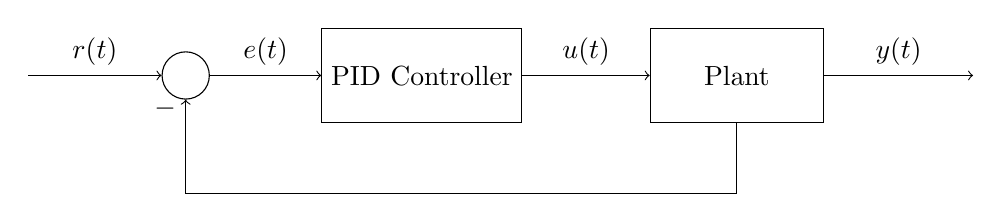
\begin{tikzpicture}[auto, node distance=2cm]

% Styles
\tikzstyle{block} = [draw, rectangle, minimum height=1.2cm, minimum width=2.2cm]
\tikzstyle{sum}   = [draw, circle, inner sep=0pt, minimum size=6mm]
\tikzstyle{input} = [coordinate]
\tikzstyle{output}= [coordinate]

% Nodes
\node [input, name=r] {};
\node [sum, right of=r] (sum) {};
\node [block, right of=sum,node distance=3cm] (pid) {PID Controller};
\node [block, right of=pid, node distance=4cm] (plant) {Plant};
\node [output, right of=plant, node distance=3cm] (y) {};

% Feedback
\node [coordinate, below of=plant, node distance=1.5cm] (fb) {};

% Connections
\draw [->] (r) -- node {$r(t)$} (sum);
\draw [->] (sum) -- node {$e(t)$} (pid);
\draw [->] (pid) -- node {$u(t)$} (plant);
\draw [->] (plant) -- node {$y(t)$} (y);
\draw [->] (plant) |- (fb) -| node[pos=0.95] {$-$} (sum);

\end{tikzpicture}
\caption{PID control system block diagram}
\end{figure}

\subsubsection{Gains}

\subsubsection*{Proportional Gain}
$K_p$ defines an output proportional to the error. A large error causes a large response and vice versa. If $K_p$ is increased, then the feedback is more sensitive to the state error. Therefore, a large proportional gain can cause overshoot. If $K_i$ and $K_d$ are not present, then the system typically doesn't reach the desired state and leaves an offset between the actual and desired state.

\subsubsection*{Integral Gain}
From a time perspective, if the proportional gain is viewed as the present, then the integral term represents the past - the previous state errors accumulate and affect the outcome. This fixes the problem with the offset, however it can also cause oscillation and slow down the response time.

\subsubsection*{Derivative Gain}
$K_d$ is not always used, but it can help dampen overshoot and oscillation. It predicts the error change as a derivative, depending on how quickly the error changes. It is highly susceptible to noise (hence why it is sometimes omitted).


\end{document}
